\documentclass{article}
\usepackage[utf8]{inputenc}

\usepackage{amsthm}
\usepackage{amsmath} 
\usepackage{bbm}
\usepackage{amsfonts}
\usepackage{graphicx,color}
\usepackage[ruled, linesnumbered]{algorithm2e}
\usepackage{algorithmic}
% \usepackage[dvipsnames]{xcolor}


\usepackage{thm-restate}
\usepackage[colorlinks,linkcolor=blue,filecolor=blue,citecolor=blue,urlcolor=blue,pdfstartview=FitH,pagebackref]{hyperref}
\usepackage[nameinlink]{cleveref}


% \theoremstyle{plain}
\newtheorem{theorem}{Theorem}%[section]
%\newtheorem{corollary}[theorem]{Corollary}
\newtheorem{lem}[theorem]{Lemma}
\crefname{lem}{Lemma}{Lemmas}
\newtheorem{claim}[theorem]{Claim}
\newtheorem{observation}[theorem]{Observation}
%\newtheorem{definition}[theorem]{Definition}
%\newtheorem{conjecture}[theorem]{Conjecture}
%\newtheorem{proposition}[theorem]{Proposition}
\newtheorem{problem}{Problem}
\newtheorem{fact}[theorem]{Fact}
%\theoremstyle{remark}
%\newtheorem*{note}{Note}


% \newcommand{\Pr}{\mathbb{Pr}}
\newcommand{\eps}{\varepsilon}
\newcommand{\R}{\mathbb{R}}
\newcommand{\N}{\mathbb{N}}
\newcommand{\Z}{\mathbb{Z}}
\newcommand{\C}{\mathcal{C}}
\newcommand{\norm}[1]{\left\| #1 \right\|}
\newcommand{\NN}{\mathcal{NN}}
\newcommand{\FF}{\mathcal{F}}
\newcommand{\LL}{\mathcal{L}}
\newcommand{\DT}{\mathcal{DT}}
\newcommand{\DG}{\mathcal{DG}}

\definecolor{purple}{RGB}{150, 1, 255}
\definecolor{DarkGreen}{RGB}{70, 130, 30}

\newcommand{\blue}{{\color{blue}blue}}
\newcommand{\red}{{\color{red}red}}
\newcommand{\purple}{{\color{purple}purple}}
\newcommand{\comment}[1]{\CommentSty{{\color{DarkGreen}#1}}}


\title{Fault tolerant spanners}

\begin{document}
	
	
	\maketitle
	
	\section{Introduction}
	
	Let $\FF$ be a family of regions in the plane, which we call the fault regions. For a fault region $F\in \FF$ and a geometric graph $G$ on a point set $P$ , we define $G\ominus F$ to be the part of $G$ that remains after the points of $P$ that are contained in $F$, and all the edges of $G$ that intersect $F$ have been removed from the graph. For simplicity, we assume that a region fault $F$ does not contain its boundary, i.e., only vertices and edges intersecting the interior of $F$ will be affected.
	
	
	Let $\LL$ be a family of regions in the plane, which we call the local regions. For a local region $L\in \LL$ and a geometric graph $G$ on a point set $P$ , we define $G\mid_F$ to be the part of $G$ contained in the interior of $F$, meaning only the vertices and edges that are fully containd in the interior of $F$.
	
	Formally, given $G=(P,E)$:
	
	$$G\ominus F = (p\setminus F, \{e\in E~|~ e\cap F = \emptyset\})$$
	$$G\mid_F = (p \cap F, \{e\in E~|~ e\subseteq F\})$$
	
	\paragraph{The problems:}
	\begin{enumerate}
		\item Given a set $P$ of points in $\R^2$, and a family $\FF$ of regions, compute a graph $G$ such that $G\ominus F$ is a $t$-spanner of $P$ for any fault $F\in\FF$
		\item Given a set $P$ of points in $\R^2$, and a family $\LL$ of regions, compute a graph $G$ such that $G\mid_F$ is a $t$-spanner for any local region $L\in\LL$
	\end{enumerate}
	.

	
	\section{Complement of disk faults / disk local spanners}
	
	
	\section{Convex faults / disk local spanners}
	Let $\FF$ be the set of convex regions, and $\eps>0$. We use the construction of Abam et al. \cite{AbamBFG09} in order to create a $(1+\eps)$-$\FF$ tolerant spanner. In their paper, Abam et al. build a \emph{semi separated pair decomposition} (SSPD), and add a set of carefully chosen edges between every two sets $A,B\subseteq P$ that compose a pair in the SSPD. Given a pair $(A,B)$, the algorithm partitions the larger set, w.l.o.g it is $B$, by shooting rays at fixed angular intervals from a disk that contains $A$, and then adds a planar set of edges $E_i$ between the convex hulls of $A$ and every part $B$ of $B$, that has the following property:
	
	For any half-plane $H$ such that $A\cap H\neq \emptyset$ and $B\cap H\neq \emptyset$, there exists an edge $e\in E_i$ such that $e\subseteq H$. This property, together with the properties of the SSPD, makes the resulted graph an $\FF$-fault tolerant spanner.
	
	We notice, that a similar construction that chooses $E_i$ to be the edges of the Delaunay triangulation with one end in $A$ and the other in $B$ has the same property. We now prove that for any disk $d\subseteq \R^2$, and for any set $P'$ of points we have that $\DT(P')\mid_d$ is connected. This is enough as half-planes can be simulated by complements of disks.
	
	\begin{claim}
		For a set of points $P\subseteq \R^2$ and for any disk $d$, $\DT(P)\mid_d$ is connected.
	\end{claim}

	\begin{proof}
		We prove a different claim that immediately implies the desired one. Let $d$ be a disk with two points $p,q\in P$ on its boundary. Then there is a path between $p$ and $q$ in $\DT(P)\mid_d$. This is enough as for every two points $p,q$ and a disk $d$ containing them, we can get a disk $d'$ that contains $p$ and $q$ on it's boundary by moving the center of $d$ in an arbitrary direction until either of them, say $p$ is on the boundary, and them moving the center of the disk towards $p$ while shrinking the size of the disk to maintain $p$ on the boundary, until $q$ as well is on the boundary.  
		
		We prove by induction over the number points in the interior of $d$.
		
		$|d\cap (P\setminus \partial d)| = 0$: Then by construction of the Delaunay triangulation the edge $\{p,q\}$ is in $\DT(P)$ and is contained in the interior of $D$.\\
		
		$|d\cap (P\setminus \partial d)| > 0$: Let $x\in P$ be a point in the interior of $d$. We move the center of $d$ in the direction of $p$, shrinking $d$ in the process, until we get a disk $d'\subseteq d$ such that $x$ is on the boundary of $d'$. By induction there is a path between $p$ and $x$ in $\DT\mid_{d'}$, and since $\DT\mid_{d'}\subseteq \DT\mid_{d}$ we have that the same path exists in $\DT\mid_{d}$. The same proof gives us a path between $x$ and $q$ and thus we are done.
		
	\end{proof}

	Since the triangulation is planar, all of the arguments from the original paper regarding the size of the spanner hold, and we get a $(1+\eps)-\FF$ fault tolerant spanner of size $O(\eps^{-3}n\log n)$ in $O(\eps^{-2}n\log n)$ time.
	
	\section{Complement of convex faults / convex  local spanners}
	Using the same argument, we can extend the result for the case where $\LL$ is the set of all scaled and translated copies, homothets, of a convex shape $\C$. While the Delaunay triangulation is not well defined for all convex shapes, the operation of creating edges between two points $p,q\in P$ such that there exist a homothet of $\C$ that contains only $p$ and $q$ and no other point of $P$ is always well defined, and gives us a graph known as the $\C$-Delaunay graph of $P$, and denoted $\DG_{\C}(P)$. The above proof applies almost verbatim for any convex $\C$, and proves the connectivity of $\DG_{\C}(P)$ for any $L\in \LL$.
	
	We need only to define a suitable shrinking operation for convex region towards a point, which is possible, for example, by parameterizing the curve defining the region and leaving the desired point in the same coordinate of the smaller curve. So, we we get a $(1+\eps)-\LL$ local spanner of size $O(\eps^{-3}n\log n)$ in $O(\eps^{-2}n\log n)$ time.(
	
%	TODO: this is actually not true unless we know how to build \DG_{\C}(P)

%	Since the Delanay triangulation is well defined for the \emph{polygonal convex distance} (L.P. Chew and R.L. Drysdale. Voronoi diagrams based on convex distance functions.InProc. 1st Sympos. Comput. Geom., pages 234–244, ACM Press, 1985), we can use the exact same proof (again replacing only the distance function and the disk) to get an algorithm for this entire family of problems.
	
	\section{$\eps$-shadow}
	
	In this section we consider a weaker form of fault tolerance. Given a family $\LL$ of shapes, we say that $G$ is a $(\LL,\eps)$-local spanner if for any $L\in\LL$ we have that $G\mid_{L_{\eps}}$, where $L_{\eps}$ is $L$ rescaled by $(1-\eps)$, is a $t$-spanner. We call $L\setminus L_{\eps}$ the \emph{shadow} of $L$, and we say that a point $p$ is \emph{truly contained} in $L$ w.r.t. $\eps$, and denote $p\in_{\eps} L$, if $p\in L_{\eps}$. 
	
	\subsection{Bounded aspect ratio rectangles}
	Let $\LL$ be the set of axis parallel rectangles with aspect ratio at most $1<\alpha$. We repeatedly preform the algorithm for convex local spanners with rectangles of different aspect-ratio, where in the $i$-th iteration we use a rectangle with aspect ratio $\left(1+\eps\right)^i$, where $i\in\{0,...,\log_{1+\eps}(\alpha)\}$. 
	
	Let $r$ be a rectangle with aspect ratio $\alpha$, and let $(A,B)$ be a pair in an SSPD such that $A\cap r\neq \emptyset$, and $B\cap r\neq \emptyset$. We assume w.l.o.g that the height of $r$ is 1, and its width is $\alpha'\in [1,\alpha]$.

	Let $i\in \{0,...,\log_{1+\eps}(\alpha)\}$ be an index for which $\alpha' \leq (1+\eps)^i \leq \frac{\alpha}{1-\eps}$ if such an index exists, then let $r'$ be the rectangle with width $\alpha'$ and aspect ratio $(1+\eps)^i$, whose horizontal bisector coincides with that of $r$. Since $(1+\eps)^i \leq \frac{\alpha}{1-\eps}$, we have that $r\setminus r'$ is contained within the shadow of $r$, and therefore $r'$ contains points of both $A$ and $B$, from the correctness of the convex local spanner, we will have an edge between a point in $A\cap r'$ and a point in $B\cap r'$. As before, this, together with the properties of the SSPD, is enough to guarantee that the constructed graph is indeed a $(\LL, \eps)$-$t$-spanner (for the appropriate choice of the parameter $s$ of the SSPD).
	
	We are left with proving that there exists an index $i\in \{0,...,\log_{1+\eps}(\alpha)\}$ for which $\alpha' \leq (1+\eps)^i \leq \frac{\alpha}{1-\eps}$.
	
	$$\alpha' \leq (1+\eps)^i \leq \frac{\alpha}{1-\eps}$$
	
	$$\log_{1+\eps}(\alpha') \leq i \leq \log_{1+\eps}\left(\frac{\alpha}{1-\eps}\right)$$
	
	$$\log_{1+\eps}(\alpha') \leq i \leq \log_{1+\eps}(\alpha) - \log_{1+\eps}(1-\eps)$$
	
	If $\log_{1+\eps}(1-\eps)<-1$, then there must be an integer $i$ with the required properties. We now notice that $(1+\eps)^{-1}=\frac{1}{1+\eps}>(1-\eps)$ [since $1>(1-\eps)(1+\eps)=(1-\eps^2)$], and so $i$ exists.
	
	The size of the spanner is $\log_{1+\eps}(\alpha)$ times the number of edges in a convex local spanner, and since $\log_{1+\eps}(\alpha)=O\left(\frac{\log(\alpha)}{\eps}\right)$, we have a spanner of size $O\left(\frac{\log(\alpha)}{\eps (t-1)^{-3}}n\log n\right)$
	
	
	\subsection{Arbitrary rectangles}
	
	In order to construct local spanners for the family $\LL$ of axis parallel rectangles with $\eps$-shadow, we describe a decomposition of the the point set $P\subseteq \R^2$ in to pairs of sets, a decomposition which we name a Quadrant Separated Pair Decomposition (QSPD). This decomposition gives us $O(n\log^2n)$ pairs $(A_i,B_i)$ of subsets of $P$, such that the sets can be separated by a vertical line and also by a horizontal line, and for every two points $p,q\in P$, there exists a single pair $(A_i,B_i)$ such that (w.l.o.g) $p\in A_i$, $q\in B_i$. This separation can be viewed as if on of the sets lies in the first quadrant of the plane (i.e. every point has positive $x$ and $y$ values), and the other is in the third quadrant (i.e. every point has negative $x$ and $y$ values), hence the name.
	
	The construction of the decomposition can be described as the repeated recursive invocation of two fairly simple subroutines denoted $S_1$ and $S_2$. The first subroutine $S_1$ goes as follows. Given a set of points $P$, and a horizontal line $l_y$, find the median of $P$ w.r.t. the $x$-coordinates of the points, and create the vertical line $l_x$ passing through it. $l_x$ and $l_y$ now divide the plane into 4 quadrants, add both pairs of diagonally opposing quadrants to the decomposition, and recurse twice, once on the points to the left of $l_x$, and once on the points to its right.
	
	The second operation is now even easier to describe. Find the median of $P$ w.r.t. the $y$-coordinates of the points, create the horizontal line $l_y$ passing through that point, call $S_1(P,l_y)$, and and recurse twice, once on the points to below of $l_y$, and once on the points above it.

	\begin{claim}
		The subroutine $S_2(P)$ creates a QSPD with size $O(n\log^2n)$.
	\end{claim}

	\begin{proof}
		By construction, each reported pair is separated w.r.t. to both dimensions, and any two point appear in diagonally opposing quadrants exactly once, as every recursive calls to both $S_1$ and $S_2$ will include only one of the points.
		
		Every call to $S_1$ creates two pairs, and generates two recursive calls, each with exactly half of the points. The formula for the size of the pairs created by $S_1$ is therefore $T(n)=2T\left( \frac{n}{2}\right) + O(n)$, which solves to $O(n)$. Very similarly, each call to $S_2$ calls $S_1$ once, and generates two recursive calls, each with exactly half of the points. The total number of pairs is therefore $S(n)=2S\left( \frac{n}{2}\right) + O(n\log n)$, which solves to $O(n\log^2n)$.
		
	\end{proof}






	We first describe a subroutine for connecting two sets of points, $A$ and $B$, where $A$ is contained in $Q^-$, the negative quadrant of the plane (i.e., have a negative value $x$-coordinate and a negative value $y$-coordinate), and $B$ is contained in $Q^+$, the positive quadrant of the plane. 
	
	Our algorithm will connect every point in $A$ to $O\left(\frac{1}{\eps^2}\right)$ points in the positive quadrant, and after performing the same process for the points of the symmetrically defined $B'$, we will have that every rectangle that truly contains points from $A$ and $B$ will have an edge $(a,b)$ with $a\in A$ and $b\in B$.
	
	For every point $a = (x',y') \in A$ we define partition the positive quadrant into $O\left(\frac{1}{\eps^2}\right)$ sets. We consider the following $\frac{1}{\eps}$ horizontal stripes - $\forall j\in \{1,...,\frac{1}{\eps}\}$:
	
	$$H_{j}:=\{(x,y)~|~  0 \leq x \leq x'+y'  ,~ (j-1)\cdot \eps y' < y \leq j\cdot \eps y'\}$$
	
	On top of these we add similarly built vertical stripes:
	
	$$V_{i}:=\{(x,y)~|~ (j-1)\cdot \eps x' < x \leq j\cdot \eps x',~ 0 \leq y \leq x'+y' \}$$
	
	These stripes create a grid which partitions the rectangle $r$ whose opposite corners are $(0,0)$ and $(|x'|,|y'|)$ into $\frac{1}{\eps^2}$ cells of width $\eps x$ and height $\eps y$. Formally:
	
	$$C_{i,j}:=\{(x',y')~|~  (i-1)\cdot \eps x < x' \leq i\cdot \eps x,~ (j-1)\cdot \eps y< y' \leq j\cdot \eps y\}$$
	
	We now divide the parts of the stripes that lie outside of the rectangle $r$. The horizontal stripes are divided into cells of width $\eps(x+y)$ and height $\eps y$, and the vertical stripes are divided into cells of width $\eps y$and height $\eps(x+y)$. The extremal cell in each stripe may be smaller if $x$ or $y$ are not divisible by $\eps(x+y)$. Formally:
	
	$$C_{H_{i,j}}:=\{(x',y')~|~  x' + (i-1)\cdot \eps (x+y) < x' \leq x' + i\cdot \eps (x+y),~ (j-1)\cdot \eps y< y' \leq j\cdot \eps y\}$$
	
	$$C_{V_{i,j}}:=\{(x',y')~|~  (i-1)\cdot \eps x < x' \leq i\cdot \eps x,~ y + (j-1)\cdot \eps (x+y)< y' \leq y + j\cdot \eps (x+y)\}$$
	
	The entire construction can be seen in Figure~\ref{fig:grid_construction}.
	
	\begin{figure}
		\centering
		\includegraphics[width=\linewidth, page=3]{grid_construction.pdf}
		\label{fig:grid_construction}
		\caption{The construction of the grid for the arbitrary axis parallel rectangle local spanner.}
	\end{figure}
	
	\begin{claim}
		For every rectangle $r\in \LL$ and a pair $(A,B)$ of the SSPD s.t. $r_{1-\eps}\cap A \neq \emptyset$ and $r_{1-\eps}\cap B \neq \emptyset$, there are two points $a\in A, b\in B$ connected by an edge.
	\end{claim}
	
	\begin{proof}
		Let $A'=A\cap r_{1-\eps}, B'=B \cap r_{1-\eps}$, and let $p= \underset{p'}{argmax}\{||p'||_{\infty}~:~ p'\in A\cup B\}$, and assume w.l.o.g that $p\in A'$ and prove that there exist a point $q\in B'$ connected to $p$ by an edge.
		
		We take a point $q'\in B'$. Due to the choice of $p$ we have that one of the coordinates of $q'$ has a smaller absolute value than the same respective coordinate of $p$, and assume w.l.o.g that it is the $x$-coordinate. Now, since $\bigcup C_{i,j} \bigcup V_i$ cover the entire part of $Q^+$ with an absolute $x$ value lower that that of $p$, we have that either there is an edge $\{p,q\}$ in the graph, or there is another point $q$ in the same cell as $q'$. Regardless, since the cells are of width $\eps\cdot p.x$ and height $\eps\cdot p.y$ ,and $r$ is of width at least $p.x$ and height at least $p.y$, we get that the entire cell is inside $r$, and therefore there exists an edge as described in the claim. 

	\end{proof}

%	We thus far have guaranteed the existence of an edge between any two sets that are separated in both the $x$ and $y$ dimensions. We now add another similar construction, whose purpose is to assure that for any two points $a,b$ in the two sets, we have a point $c$ which is connected by an edge to one of these points, and is very close to the other.
%	
%	So, as before, describe a subroutine for sets $A$ and $B$, where $A$ is contained in $Q^-$, and $B$ is contained in $Q^+$, the positive quadrant of the plane. For every point $a = (x,y) \in A$ we define partition the positive quadrant into the following $O\left(\frac{1}{\eps^2}\right)$ sets $\forall i,j\in \{1,...,\frac{1}{\eps}\}$:
%	
%	$$C_{i,j}:=\{(x',y')~|~  (i-1)\cdot \eps (x+y) < x' \leq i\cdot \eps (x+y),~ (j-1)\cdot \eps (x+y)< y' \leq j\cdot \eps (x+y)\}$$
%	
%	We add an edge between $a$ and an arbitrary point of $P$ from each $C_{i,j}$ (when such a point exists).
%	
%	\begin{claim}
%		For every rectangle $r\in \LL$ and a pair $(A,B)$ of the SSPD s.t. $r_{1-\eps}\cap A \neq \emptyset$ and $r_{1-\eps}\cap B \neq \emptyset$, there are two points $a\in A, b\in B$ connected by an edge.
%	\end{claim}
%	
%	\begin{proof}
%		Let $A'=A\cap r_{1-\eps}, B'=B \cap r_{1-\eps}$, and let $p= \underset{p'}{argmax}\{||p'||_{\infty}~:~ p'\in A\cup B\}$, and assume w.l.o.g that $p\in A'$ and prove that there exist a point $q\in B'$ connected to $p$ by an edge.
%		
%		We take a point $q'\in B'$. Due to the choice of $p$ we have that one of the coordinates of $q'$ has a smaller absolute value than the same respective coordinate of $p$, and assume w.l.o.g that it is the $x$-coordinate. Now, since $\bigcup C_{i,j} \bigcup V_i$ cover the entire part of $Q^+$ with an absolute $x$ value lower that that of $p$, we have that either there is an edge $\{p,q\}$ in the graph, or there is another point $q$ in the same cell as $q'$. Regardless, since the cells are of width $\eps\cdot p.x$ and height $\eps\cdot p.y$ ,and $r$ is of width at least $p.x$ and height at least $p.y$, we get that the entire cell is inside $r$, and therefore there exists an edge as described in the claim. 
%		
%		
%		
%	\end{proof}
	
	\subsection{Bounded aspect ratio triangles}
	
	The aspect ratio of a triangle is defined as the length of its longest edge divided by its height as it is measured from that edge. Let $\LL$ be the set of all triangles with aspect ratio at most $\alpha$ for some $1 < \alpha$. We define a set of slopes, and for each subset of 3 slopes we run the convex region algorithm with $\LL$ as homothets of a triangle with edges of the 3 chosen slopes. As long as the fixed angular interval is smaller than $\eps' = \arctan\left(\frac{\eps/2}{\alpha(1-\eps/2)}\right)$ (see figure~\ref{fig:triangle_with_shadow}).
	
	This construction creates $\frac{1}{\eps'}$ different convex local spanners, and so we get a $(1+\eps)$-local spanner for triangles with bounded aspect ratio in $O\left(\frac{1}{\eps'^3\eps^3} n\log n\right)$.

	
	\begin{figure}
		\centering
		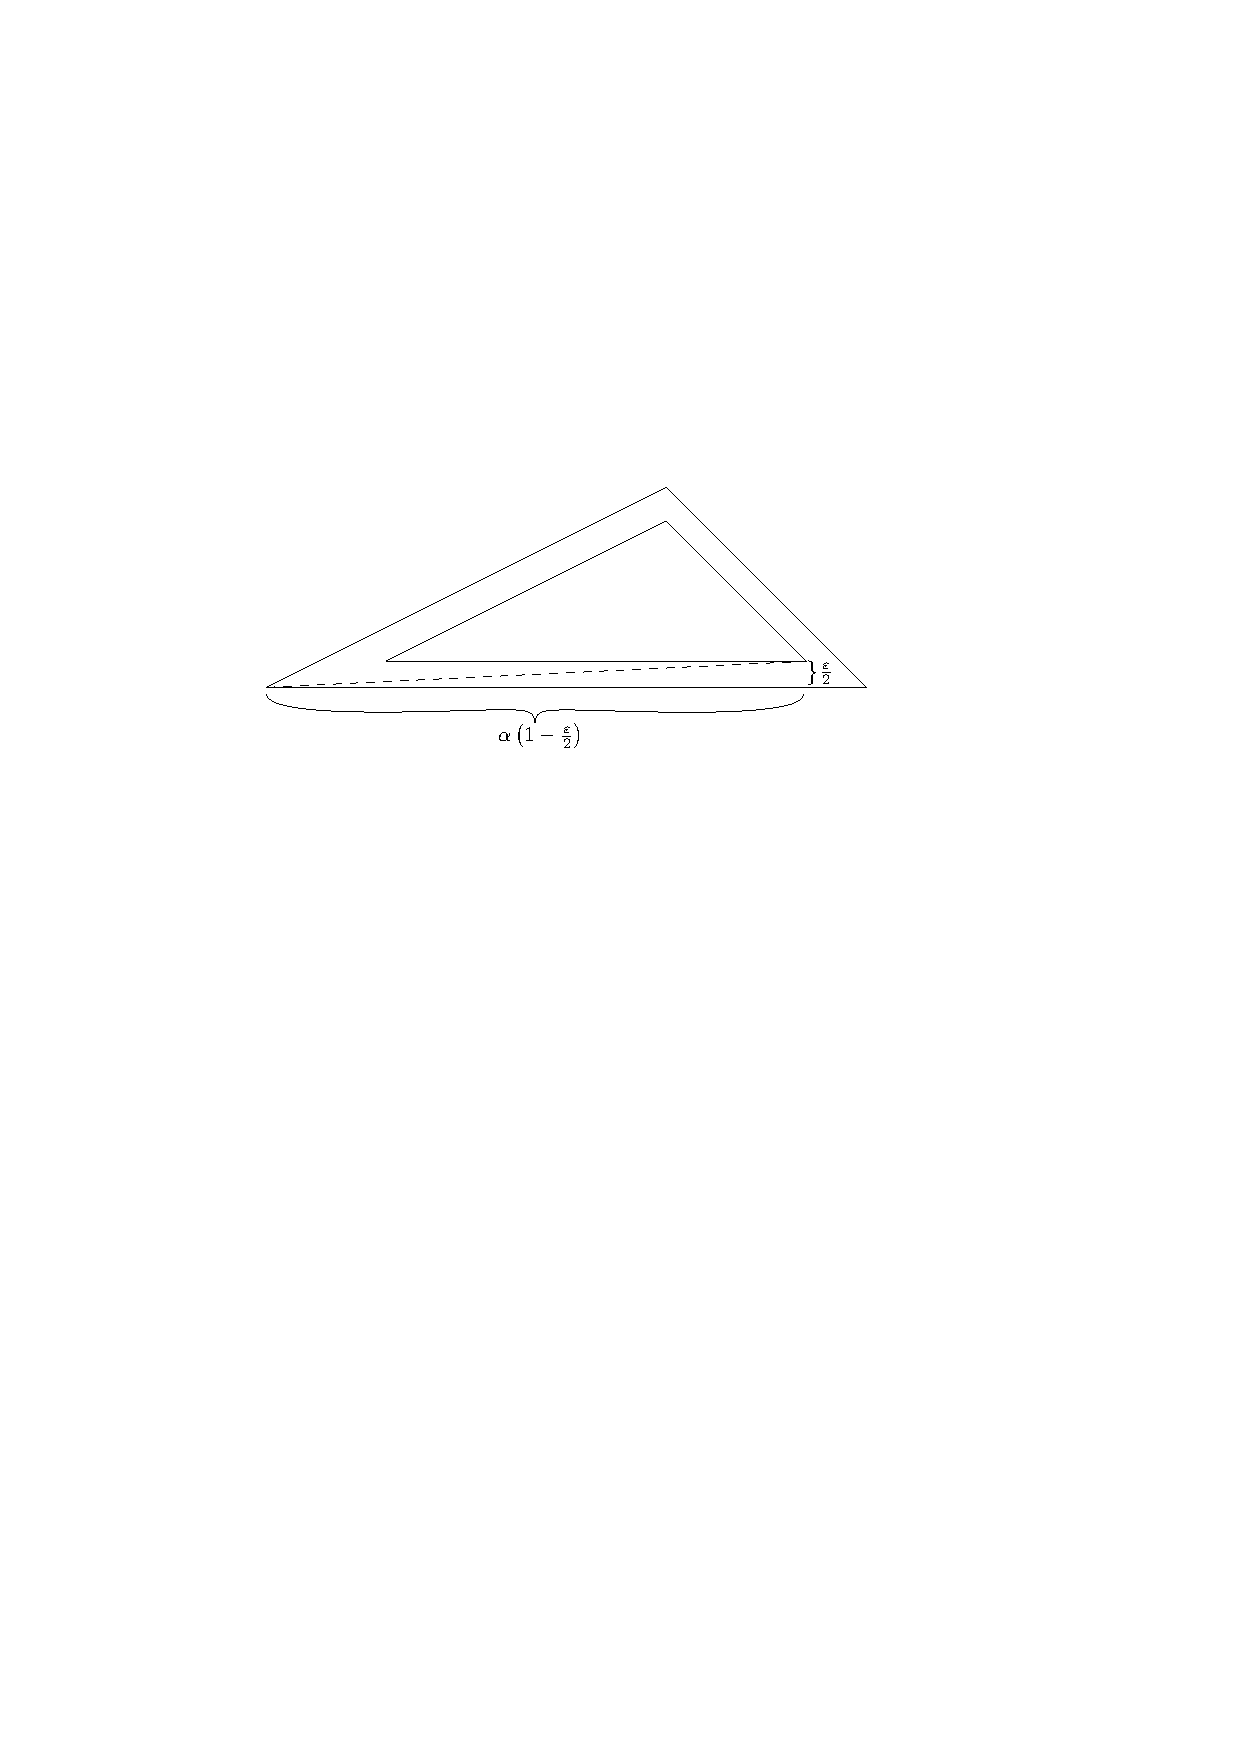
\includegraphics[width=0.6\linewidth]{triangle_shadow.pdf}
		\label{fig:triangle_with_shadow}
	\end{figure}
\bibliography{refs}

\end{document}
